\documentclass[xcolor=svgnames,t]{beamer} 
\usepackage[utf8]{inputenc}
\usepackage{booktabs, comment}
\usepackage{graphicx}  % Add graphicx package
\usepackage[absolute, overlay]{textpos} 
\usepackage{pgfpages}
\usepackage[font=footnotesize]{caption}
\useoutertheme{infolines} 
\usepackage{xcolor}
\usepackage{cite}
\usepackage{colortbl}
\definecolor{brownbrown}{RGB}{8, 8, 9}
\usepackage[round, sort, authoryear]{natbib}
\definecolor{brownred}{RGB}{198, 198, 198}

\setbeamercolor{title in head/foot}{bg=brownred, fg=brownbrown}
\setbeamercolor{author in head/foot}{bg=myuniversity}
\setbeamertemplate{page number in head/foot}{}

\usepackage{amsmath}
\usepackage[makeroom]{cancel}

\newtheorem{equi}{} %Creates a grey box when equi is called
\setbeamertemplate{navigation symbols}{} 
\usepackage{textpos}

\usepackage{tikz}

\usetheme{Madrid}
\definecolor{myuniversity}{RGB}{48, 67, 180}
\usecolortheme[named=myuniversity]{structure}
\usepackage{tikz}

\newcommand{\myitem}{\item[$\circ$]}
\newcommand{\witem}{\item[\textcolor{white}{$\bullet$}]}
\DeclareMathOperator*{\argmax}{arg\,max}
\DeclareMathOperator*{\argmin}{arg\,min}
\AtBeginSection[]{
\begin{frame}
\frametitle{Content}
\tableofcontents[currentsection]
\end{frame}
}

\title[Introduction to Causal Inference]{Introduction to Causal Inference}
\subtitle{}
%\titlegraphic{\includegraphics[height=1cm]{brown-logo.png}}  % This line is commented out to remove the logo
\author[CIML 2024]{Causal Inference using Machine Learning\\ Master in Economics, UNT}
\institute[]{Andres Mena}
\date{Spring 2024}

\addtobeamertemplate{navigation symbols}{}{%
    \usebeamerfont{footline}%
    \usebeamercolor[fg]{footline}%
    \hspace{1em}%
    \insertframenumber/\inserttotalframenumber
}

\begin{document}
\begin{frame}
\maketitle
\end{frame}

%%%%%%%%%%%%%%%%%%%%%%%%%%%%
%\logo{\includegraphics[height=0.5cm]{brown-arms.png}}  % This line is commented out to remove the logo
%%%%%%%%%%%%%%%%%%%%%%%%%%

\begin{frame}
    \frametitle{Table of Contents}
    \tableofcontents
\end{frame}

\section{What is Causal Inference?}
\begin{frame}
    \frametitle{What is a Causal Question?}
    
    % Show the image first
    \begin{center}
    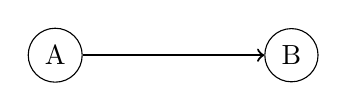
\begin{tikzpicture}
        \node[draw, circle] (A) at (0,0) {A};
        \node[draw, circle] (B) at (3,0) {B};
        \draw[->, thick] (A) -- (B);
    \end{tikzpicture}
    \end{center}
    
    \pause % Transition to the bullet points
    
    A causal question asks about the effect of a cause \(A\) on an outcome \(B\).
    
    \pause % Transition to the first main bullet
    \begin{itemize}
        \item \(A\) could be: % Introduce sub-bullets for A
        \begin{itemize}
            \pause
            \item Policy (e.g., a new transfer policy impacting household income (AUH))
            \pause
            \item Treatment (e.g., a drug trial reducing heart attack risk)
            \pause
            \item Business strategy (e.g., a marketing campaign affecting sales)
            \pause
            \item Technological innovation (e.g., the introduction of innovation of supply chain)
        \end{itemize}
        
        \pause % Transition to the second main bullet
        \item \(B\) could be: % Single item + example for B
        \begin{itemize}
            \pause
            \item Welfare (e.g., income, poverty, crime, happiness, inequality)
            \pause
            \item Health (e.g., life expectancy, disease risk, heart attacks)
            \pause
            \item Profits (e.g., company earnings,  market share, costs)
            \pause
            \item Efficiency (e.g., speed of production or resource utilization)
        \end{itemize}
    \end{itemize}
\end{frame}



\begin{frame}
    \frametitle{Correlation is not Causation (and vice versa)}

    \textbf{1. Correlation \(\cancel{\rightarrow}\) Causation}
    
    \pause % Transition to correlation definition
    
    \begin{itemize}
        \item \textbf{Correlation}: A statistical relationship between two variables, where changes in one variable are associated with changes in another. 
        \[
        \text{Corr}(A, B) = \frac{\text{Cov}(A, B)}{\sigma_A \sigma_B}
        \]
    \end{itemize}
    
    \pause % Transition to correlation example
    
    \begin{itemize}
        \item Example: Rain and umbrellas. 
    \end{itemize}

    \pause % Transition to the causation part

    \textbf{2. Causation \(\cancel{\rightarrow}\) Correlation}

    \pause % Transition to causation definition
    
    \begin{itemize}
        \item \textbf{Causation}: A direct effect of one variable on another, where \(A\) causes \(B\).
        \[
        B = f(A)
        \]
    \end{itemize}
    
    \pause % Transition to causation example
    
    \begin{itemize}
        \item Example: Eating more food can cause weight gain, but if food intake and exercise both increase proportionally, we may observe no correlation between food and weight in the data, even though causation exists.
    \end{itemize}

\end{frame}

\begin{frame}
    \frametitle{Causal Inference Tree}
    \begin{figure}
        \includegraphics[width=0.8\linewidth]{Figures/CI_tree.jpg}
        \caption{Source: Scott Cunningham Substack}
    \end{figure}
\end{frame}


\begin{frame}
    \frametitle{Experimental Design Tradition}
    
    Experimental design relies on randomized controlled trials (RCTs) to establish causality through direct manipulation of the treatment.

    \begin{itemize}
        \item \textbf{Neyman (1923)}: 
        \begin{itemize}
            \item Introduced the concept of randomization in experiments and formalized the \textbf{potential outcomes} framework.
            \item \textit{Contribution}: Randomization as a tool to eliminate bias.
        \end{itemize}
        
        \pause % Transition to Rubin
        \item \textbf{Rubin (1974)}: 
        \begin{itemize}
            \item Developed the potential outcomes model in the context of randomized experiments.
            \item \textit{Contribution}: Introduced the Rubin Causal Model (RCM) as a framework for understanding causal effects.
        \end{itemize}
        
        \pause % Transition to Duflo
        \item \textbf{Esther Duflo (Nobel Prize 2019)}: 
        \begin{itemize}
            \item Pioneered the use of randomized controlled trials in development economics to study policy interventions.
            \item \textit{Contribution}: Applied RCTs to measure the effectiveness of educational and poverty interventions in developing countries.
        \end{itemize}
    \end{itemize}

\end{frame}

\begin{frame}
    \frametitle{Quasi-experimental Design}
    
    \small % Reducing font size to fit the text
    Quasi-experimental designs use natural variation and perform comparisons under assumptions.
    \pause 
    \begin{itemize}
        \item \textbf{Difference-in-Differences (DiD)}: 
        \begin{itemize}
            \item \textbf{John Snow's Cholera Study (1854)}: Snow used natural variation in water sources to compare cholera outcomes between neighborhoods \citep{snow1854}.
            \item \textit{Causal Question}: Does contaminated water cause cholera?
        \end{itemize}
        
        \pause % Transition to IV
        \item \textbf{Instrumental Variables (IV)}: 
        \begin{itemize}
            \item \textbf{Wright (1928)}: Used supply-side instruments to estimate demand for agricultural products \citep{wright1928}.
            \item \textit{Causal Question}: What is the causal effect of price on the quantity demanded?
        \end{itemize}
        
        \pause % Transition to RD
        \item \textbf{Regression Discontinuity (RD)}: 
        \begin{itemize}
            \item \textbf{Thistlethwaite and Campbell (1960)}: Studied the effect of merit awards on student performance \citep{thistlethwaite1960}.
            \item \textit{Causal Question}: What is the effect of winning a merit award on future academic success?
        \end{itemize}
        
        \pause % Transition to SCM
        \item \textbf{Synthetic Control (SCM)}: 
        \begin{itemize}
            \item \textbf{Abadie et al. (2010)}: Developed SCM to evaluate the effects of California’s Tobacco Control Program \citep{abadie2010}.
            \item \textit{Causal Question}: What is the effect of California’s anti-tobacco policies on smoking rates?
        \end{itemize}
    \end{itemize}
\end{frame}
\section{The Four Questions of Causal Inference}
\section{Probability Essentials}
\section{Treatment Effects definitions}
\begin{frame} [allowframebreaks]
    \frametitle{References}
    \bibliographystyle{apalike}
    \bibliography{references}
\end{frame}

\end{document}


































 


